\documentclass{beamer}
\usetheme{Darmstadt}
\usecolortheme{beaver}

% Custom colors
\definecolor{bgsubrown}{RGB}{79,44,29}
\definecolor{bgsuorange}{RGB}{253,80,0}
\setbeamercolor{structure}{fg=bgsubrown}
\setbeamercolor{title}{fg=bgsuorange,bg=bgsubrown}
\setbeamercolor{frametitle}{fg=bgsuorange,bg=bgsubrown}
\setbeamercolor{alerted text}{fg=bgsuorange}
\setbeamercolor{section in toc}{fg=bgsuorange}
\setbeamercolor{subsection in toc}{fg=bgsuorange}
\setbeamercolor{section in head/foot}{fg=bgsuorange}
\setbeamercolor{subsection in head/foot}{fg=bgsuorange}


% Essential packages only
\usepackage{booktabs}
\usepackage{colortbl}
\usepackage{multicol}
\usepackage{tikz}
\usepackage{calligra}

% Beamer settings
\setbeamertemplate{footline}[frame number]
\setbeamertemplate{navigation symbols}{}
\setbeamercovered{transparent=0} % keeps images from being covered with \pause

% Start of slides
\title{Predicting Learning Commons Usage:\\Duration and Occupancy}
\subtitle{A Non-Linear Approach}
\author{Naiyue Liang (Emma), Ryan Renken, Jaryt Salvo, \& Jason Turk}
\institute{MATH 7560 Statistical Learning II \textbar\textbar \space BGSU}
\date{\today}

\begin{document}

\begin{frame}
\titlepage
\end{frame}


\section{Kmeans++}

\begin{frame}
\frametitle{K-means: Data \& Motivation}
    % \textbf{Data}: Points sampled from a small subset of \(\mathbb{R}^2\).

    % \vspace{0.5em} % Small space before alert block
    \begin{alertblock}{Clustering Task}
        \small % Keep text size small inside block
        \begin{itemize}
            \item \textbf{Goal}: Partition \(\mathbb{R}^2\) data into \(k=11\) clusters.
            \item \textbf{Comparison}: Standard K-means vs K-means++ initialization.
            \item \textbf{K-means++ Motivation}: Better initial centroids for potentially faster/better clustering.
        \end{itemize}
    \end{alertblock}

    \vspace{0.5em} % Add vertical space before the image
    \begin{center}
        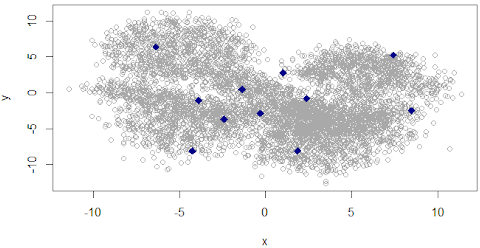
\includegraphics[width=0.8\textwidth]{images/kmeans/kmeanscloud.png}
    \end{center}
\end{frame}

\begin{frame}
\frametitle{K-means vs K-means++ Results}
    \vspace{1em}
    \begin{columns}[T] % Align columns at the top
        \column{0.4\textwidth}
        \small % Use smaller font for text
        \textbf{Standard K-means}:
            \begin{itemize}
            \item \textbf{Stats}: 5 iterations, WCSS = 22,824.
            \end{itemize}

        \vspace{1em} % Add more vertical space between the two stat blocks

        \textbf{K-means++ Initialization}:
        \vspace{-1em}
            \begin{itemize}
            \item \textbf{Stats}: 8 iterations, WCSS = 22,943.
            \end{itemize}
        
        \begin{alertblock}{Observation}
            K-means++ offered no clear advantage over standard K-means for this dataset (visually or by WCSS).
        \end{alertblock}
    

        \column{0.65\textwidth}
        \centering % Center the images
        \vspace{-2em}
        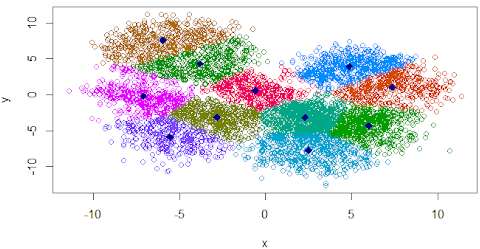
\includegraphics[width=\textwidth, height=0.55\textheight]{images/kmeans/kmeans.png} \\
        \vspace{-1em} % Space between images
        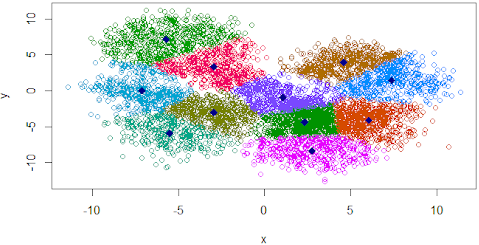
\includegraphics[width=\textwidth, height=0.55\textheight]{images/kmeans/kmeanspp.png}
    \end{columns}
    
\end{frame}



\section{Learning Commons Data}

% \begin{frame}
% \frametitle{Data Overview}
%     \begin{columns}
%         \column{0.6\textwidth}
%         \textbf{Dataset Characteristics}:
%             \begin{itemize}
%             \item Learning Commons visit records
%             \item \textbf{Train}: Fall 2016 - Spring 2017
%             \item \textbf{Test}: Fall 2017 - Spring 2018
%             \item Two prediction tasks:
%                 \begin{itemize}
%                 \item Visit Duration (in minutes)
%                 \item Occupancy at check-in
%                 \end{itemize}
%             \end{itemize}
            
%         \textbf{Key Features}:
%             \begin{itemize}
%             \item Student demographics
%             \item Academic performance metrics
%             \item Course information
%             \item Temporal visit data
%             \end{itemize}
                
%         \column{0.4\textwidth}
%         \begin{alertblock}{Prediction Tasks}
%             \begin{itemize}
%             \item Part A: Predict Duration\_In\_Min
%             \item Part B: Predict Occupancy
%             \end{itemize}
%         \end{alertblock}
%     \end{columns}
% \end{frame}

\begin{frame}
    \frametitle{Distribution Statistics}
        \begin{columns}[T]
            \column{0.4\textwidth}            
            \vspace{-0.2cm}
            \footnotesize{\textbf{Duration (minutes)}:}
            \vspace{-0.2cm}
            \begin{center}
            \footnotesize
            \begin{tabular}{>{\columncolor{bgsubrown!20}}l r}
            \toprule
            \textbf{Statistic} & \textbf{Value} \\
            \midrule
            Minimum & 6.00 \\
            1st Quartile & 44.00 \\
            Median & 68.00 \\
            Mean & 81.78 \\
            3rd Quartile & 103.00 \\
            Maximum & 822.00 \\
            \bottomrule
            \end{tabular}
            \end{center}
            
            \footnotesize{\textbf{Occupancy (students)}:}
            \vspace{-0.2cm}
            \begin{center}
            \footnotesize
            \begin{tabular}{>{\columncolor{bgsubrown!20}}l r}
            \toprule
            \textbf{Statistic} & \textbf{Value} \\
            \midrule
            Minimum & 1.00 \\
            1st Quartile & 7.00 \\
            Median & 11.00 \\
            Mean & 11.62 \\
            3rd Quartile & 15.00 \\
            Maximum & 40.00 \\
            \bottomrule
            \end{tabular}
            \end{center}
                
            \column{0.6\textwidth}
            % \footnotesize{\textbf{Distribution Plots}:}
            \vspace{0.2cm}
            
            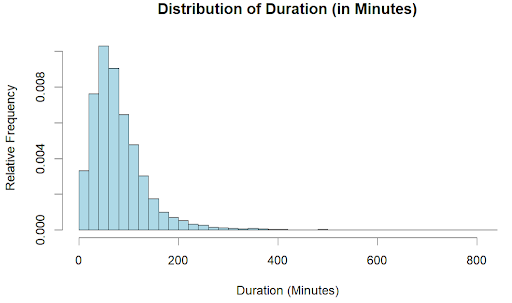
\includegraphics[width=\textwidth, height=0.46\textheight]{images/eda/dist_duration.png}
            \vspace{0.3cm}
            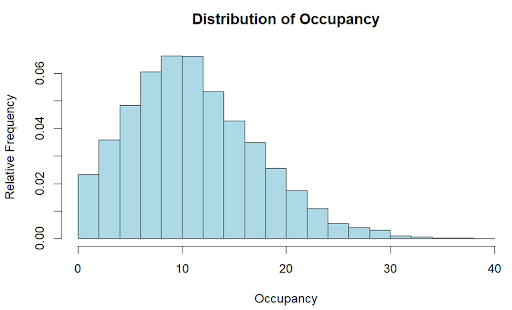
\includegraphics[width=\textwidth, height=0.41\textheight]{images/eda/dist_occupancy.png}
        \end{columns}
    
        \begin{alertblock}{Key Insight}
            Both distributions show right-skewed patterns, with some extreme values particularly in duration.
        \end{alertblock}
\end{frame}


% \section{Feature Engineering}

\begin{frame}
\frametitle{Feature Categories Overview}
    \begin{center}
    \small
    \begin{tabular}{>{\columncolor{bgsubrown!20}}l l}
    \toprule
    \textbf{Category} & \textbf{Key Features} \\
    \midrule
    Temporal & Time of day, Day of week, Week of semester \\
    \midrule
    Academic & Course level, GPA categories, Credit load \\
    \midrule
    Visit & Duration patterns, Group sizes, Visit frequency \\
    \midrule
    Course & Subject areas, Level progression, Course mix \\
    \midrule
    Student & Major groups, Class standing, Academic progress \\
    \bottomrule
    \end{tabular}

    \vspace{1em} % Add space between tables

    \hspace*{-1em} % Shift this table slightly left
    \begin{tabular}{>{\columncolor{bgsubrown!20}}m{0.3\textwidth} >{\arraybackslash}m{0.7\textwidth}}
    \toprule
    \textbf{External Source} & \textbf{Key Features} \\
    \midrule
    R library `lunar` & Moon phase data \\
    \midrule
    R library `openmeteo` & Hourly weather metrics (temperature, humidity, pressure, cloud cover, wind, radiation, precipitation, \& soil conditions) \\
    \bottomrule
    \end{tabular}
    \end{center}
\end{frame}    

\begin{frame}
\frametitle{Dropped Raw Features}
    \noindent
    \hspace{-1cm}
    % \begin{center}
    \small
    \begin{tabular}{>{\columncolor{bgsubrown!20}}l l}
    \toprule
    \textbf{Raw Feature} & \textbf{Engineered Into} \\
    \midrule
    Student\_IDs & Total\_Visits, Semester\_Visits, Avg\_Weekly\_Visits \\
    \midrule
    Class\_Standing & Class\_Standing\_Self\_Reported, Class\_Standing\_BGSU \\
    \midrule
    Major & Major\_Category, Has\_Multiple\_Majors \\
    \midrule
    Expected\_Graduation & Expected\_Graduation\_Date, Months\_Until\_Graduation \\
    \midrule
    Course\_Name & Course\_Name\_Category \\
    \midrule
    Course\_Number & Unique\_Courses, Course\_Level\_Mix \\
    \midrule
    Course\_Type & Course\_Type\_Category \\
    \midrule
    Course\_Code\_by\_Thousands & Course\_Level, Advanced\_Course\_Ratio \\
    \midrule
    \end{tabular}
    % \end{center}

    \begin{alertblock}{Feature Engineering Strategy}
        Raw features were transformed into more informative derived features, capturing higher-level patterns and relationships in the data.
    \end{alertblock}
\end{frame}

% \begin{frame}
% \frametitle{Complete Feature List (\url{~}50 Pre-Dummied)}
%     % \begin{center}
%     \noindent
%     \hspace{-1cm}
%     \footnotesize
%     \begin{tabular}{>{\columncolor{bgsubrown!20}}m{0.16\textwidth} >{\arraybackslash}m{0.93\textwidth}}
%     \toprule
%     \textbf{Category} & \textbf{Features} \\
%     \midrule
%     Student Demographics & \textbf{Student\_IDs}, Gender, \textbf{Class\_Standing}, Class\_Standing\_Self\_Reported, Class\_Standing\_BGSU, Has\_Multiple\_Majors, \textbf{Major}, Major\_Category, Degree\_Type \\
%     \midrule
%     Academic Performance & \textbf{Total\_Credit\_Hours\_Earned}, Term\_Credit\_Hours, Credit\_Load\_Category, Term\_GPA, Cumulative\_GPA, Change\_in\_GPA, GPA\_Category, GPA\_Trend \\
%     \midrule
%     Course Information & \textbf{Course\_Name}, \textbf{Course\_Number}, \textbf{Course\_Type}, Course\_Type\_Category, Course\_Level, \textbf{Course\_Code\_by\_Thousands}, Course\_Name\_Category, Course\_Level\_Mix, Advanced\_Course\_Ratio, Unique\_Courses \\
%     \midrule
%     Temporal Features & \textbf{Check\_In\_Time}, \textbf{Check\_Out\_Time}, \textbf{Check\_In\_Date}, Check\_In\_Hour, Check\_In\_Day, Check\_In\_Month, \textbf{Semester}, Semester\_Week, Check\_In\_Week, Is\_Weekend, Time\_Category \\
%     \midrule
%     Visit Metrics & \underline{\textbf{Duration\_In\_Min}}, Group\_Size, Group\_Size\_Category, Group\_Check\_In, Total\_Visits, Semester\_Visits, Week\_Volume, Avg\_Weekly\_Visits, \underline{\textbf{Occupancy}} \\
%     \midrule
%     Graduation & \textbf{Expected\_Graduation}, Expected\_Graduation\_Date, Months\_Until\_Graduation \\
%     \bottomrule
%     \end{tabular}
%     % \end{center}

%     \begin{alertblock}{Feature Set}
%         Total of 48 features used for model training, organized into logical categories.
%     \end{alertblock}
% \end{frame}


\section{Model Building}

\begin{frame}
\frametitle{Model Hyperparameter Tuning Ranges}
    \vspace{-1em} % Reduce space below title
    \begin{columns}[T] % Align columns at the top
        \hspace*{-1.5em}
        \column{0.5\textwidth}
        \centering % Center content in the column
        \textbf{Duration Task Models} \vspace{0.5em} \\ % Title for first table
        \small % Use smaller font for tables
        \begin{tabular}{>{\columncolor{bgsubrown!20}}m{0.3\textwidth} >{\arraybackslash}m{0.65\textwidth}}
        \toprule
        \textbf{Model} & \textbf{Hyperparameters} \\
        \midrule
        MARS & \textbf{num\_terms}: \([7, 15]\) \newline \textbf{prod\_degree}: 1 \\
        \addlinespace[0.5em]
        Random Forest & \textbf{trees}: \([300, 325]\) \newline \textbf{min\_n}: \([15, 25]\) \newline \textbf{mtry}: \([20, 25]\) \\
        \addlinespace[0.5em]
        XGBoost & \textbf{trees}: \([75, 100]\) \newline \textbf{tree\_depth}: \([15, 21]\) \newline \textbf{learn\_rate}: 0.05 \newline \textbf{min\_n}: \([10, 15]\) \newline \textbf{mtry}: \([12, 15]\) \\
        \bottomrule
        \end{tabular}
        
        \column{0.5\textwidth}
        \centering % Center content in the column
        \textbf{Occupancy Task Models} \vspace{0.5em} \\ % Title for second table
        \small % Use smaller font for tables
        \begin{tabular}{>{\columncolor{bgsubrown!20}}m{0.3\textwidth} >{\arraybackslash}m{0.65\textwidth}}
        \toprule
        \textbf{Model} & \textbf{Hyperparameters} \\
        \midrule
        MARS & \textbf{num\_terms}: \([120, 130]\) \newline \textbf{prod\_degree}: 1 \\
        \addlinespace[0.5em]
        Random Forest & \textbf{trees}: \([250, 350]\) \newline \textbf{min\_n}: \([2, 3]\) \newline \textbf{mtry}: \([40, 45]\) \\
        \addlinespace[0.5em]
        XGBoost & \textbf{trees}: \([350, 450]\) \newline \textbf{tree\_depth}: \([6, 8]\) \newline \textbf{learn\_rate}: 0.1 \newline \textbf{min\_n}: \([2, 3]\) \newline \textbf{mtry}: \([30, 35]\) \\
        \bottomrule
        \end{tabular}
    \end{columns}

    % \begin{alertblock}{Implementation Details}
    %     \vspace{-0.3cm}
    %     \small
    %     \begin{columns}
    %         \column{0.55\textwidth}
    %         \begin{itemize}
    %             \setlength{\itemsep}{0pt}
    %             \item \textbf{Duration}: Log-normal
    %             \item \textbf{Occupancy}: Poisson \& Weibull
    %             \item Integer rounding for occupancy
    %         \end{itemize}

    %         \column{0.45\textwidth}
    %         \begin{itemize}
    %             \setlength{\itemsep}{0pt}
    %             \item Grid search optimization
    %             \item Feature selection
    %             \item Cross-validation
    %         \end{itemize}            
    %     \end{columns}
    % \end{alertblock}
    
\end{frame}

% \begin{frame}
% \frametitle{Task-Specific Models}
%     \begin{columns}%[T]
%         \vspace{-1cm}
%         \column{0.5\textwidth}
%         % \begin{center}
%         \small
%         \begin{tabular}{>{\columncolor{bgsubrown!20}}p{0.3\textwidth} p{0.6\textwidth}}
%         \toprule
%         \textbf{Duration Model} & \textbf{Hyperparameters} \\
%         \midrule
%         Penalized-LogNormal & \textbf{link}: log1p, \\
%         & \textbf{ridge}: $\alpha \in [10^0, 10^2]$ \\
%         \bottomrule
%         \end{tabular}
        
%         \vspace{0.2cm}
        
%         \begin{tabular}{>{\columncolor{bgsubrown!20}}m{0.3\textwidth} m{0.6\textwidth}}
%         \toprule
%         \textbf{Occupancy Models} & \textbf{Hyperparameters} \\
%         \midrule
%         Penalized-Poisson & \textbf{link}: log + exp \newline
%                            \textbf{ridge}: $\alpha \in [10^0, 10^2]$ \\
%         \addlinespace[0.5em]
%         Penalized-Weibull & \textbf{link}: (\(\ln(-\ln(1 - F(x)))\)) \newline
%                            \textbf{ridge}: $\alpha \in [10^0, 10^2]$ \\
%         \bottomrule
%         \end{tabular}
%         % \end{center}
            
%         \column{0.5\textwidth}
%         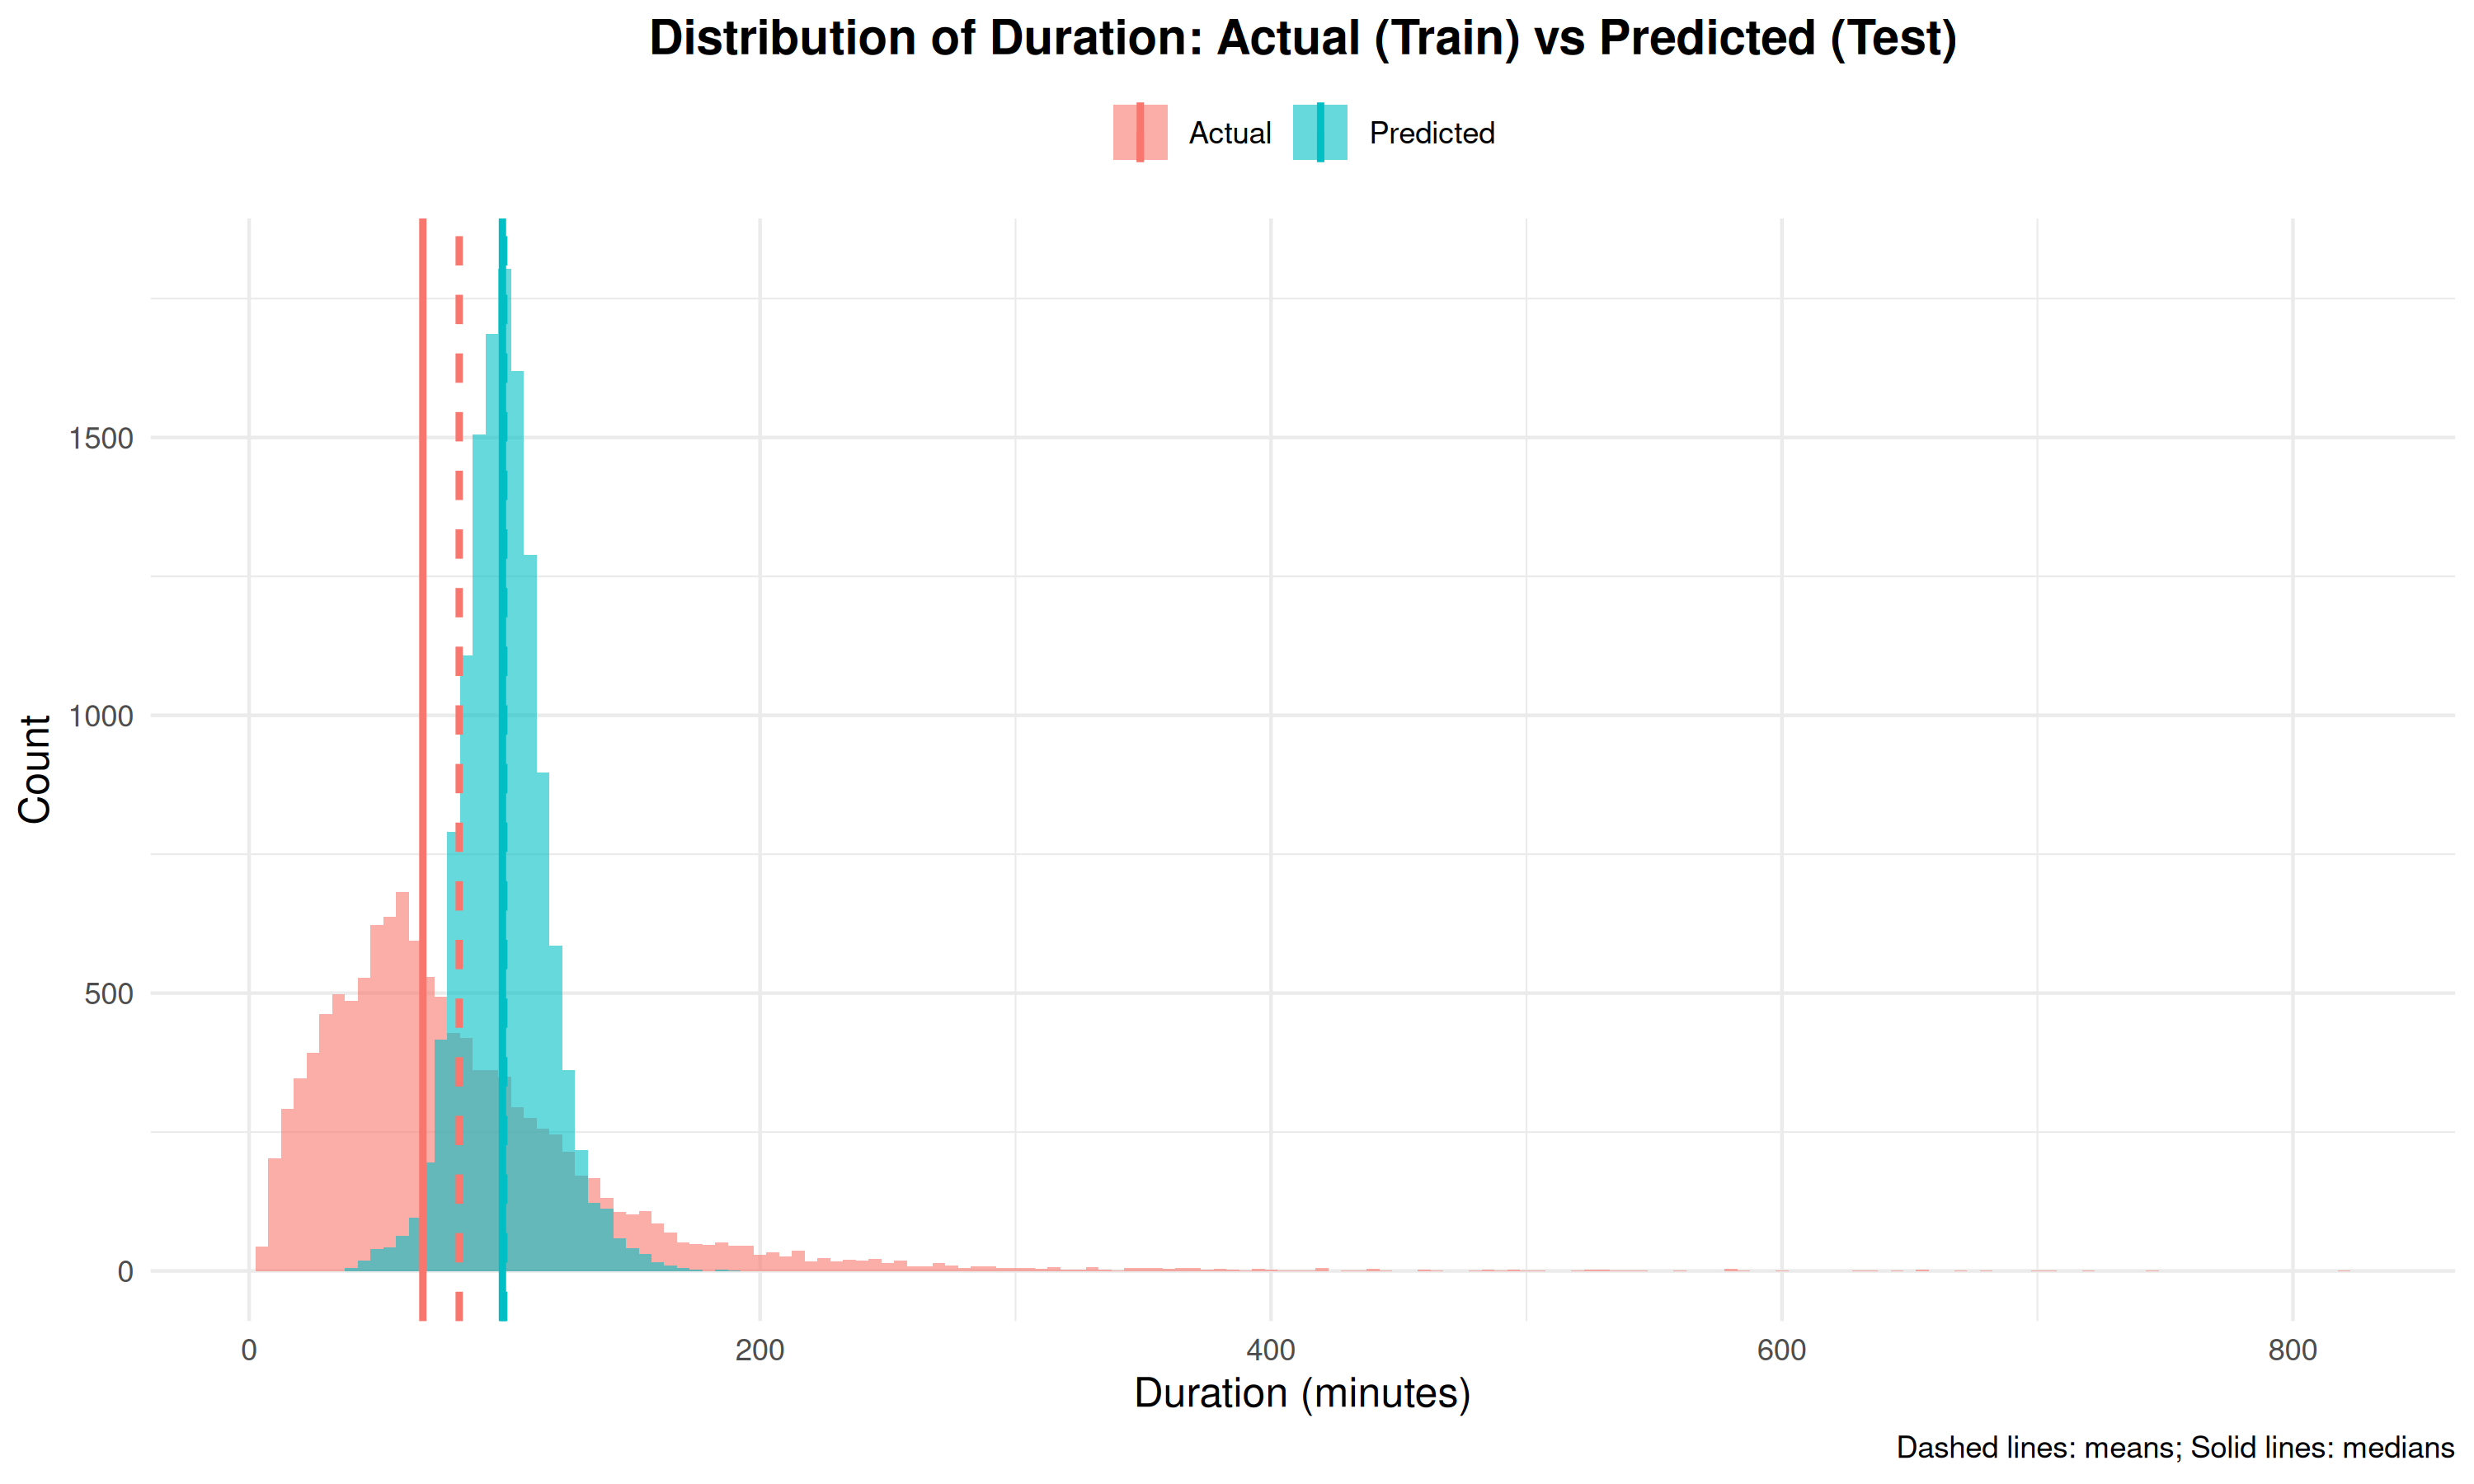
\includegraphics[width=\textwidth]{images/eda/duration_distribution.png}
%     \end{columns}

%     \begin{alertblock}{Task-Specific Implementation}
%         \begin{itemize}
%             \item Duration: k $\in [10, 50]$ features, log-normal transform for skewness
%             \item Occupancy: k $\in [70, 100]$ features, rounded integer predictions
%         \end{itemize}
%     \end{alertblock}
% \end{frame}

\begin{frame}
\frametitle{Model Pipeline Configurations}
    \raggedright
    \hspace*{-1.5cm} % Negative horizontal space to move leftwards
    \begin{columns}            
        \column{0.48\textwidth}
        \small
        \begin{tabular}{>{\columncolor{bgsubrown!20}}l l}
        \toprule
        \textbf{CV Method} & \textbf{Description} \\
        \midrule
        kfold & Random k splits \\
        \midrule
        rolling & Fixed-size window \\
        & moving forward \\
        \midrule
        expanding & Growing window with \\
        & fixed start point \\
        \bottomrule
        \end{tabular}

        \column{0.5\textwidth}
        \small
        \setlength{\parindent}{0pt}
        \begin{tabular}{>{\columncolor{bgsubrown!20}}p{0.25\textwidth} p{0.7\textwidth}}
        \toprule
        \textbf{Pipeline} & \textbf{Implementation} \\
        \midrule
        vanilla & Scaling $\rightarrow$ Model \\
        \midrule
        interact & Scaling $\rightarrow$ Interactions \\
        \_select & $\rightarrow$ SelectKBest $\rightarrow$ Model \\
        \midrule
        & Scaling $\rightarrow$ PCA/LDA \\
        pca\_lda & $\rightarrow$ Interactions \\
        & $\rightarrow$ SelectKBest $\rightarrow$ Model \\
        \bottomrule
        \end{tabular}
    \end{columns}

    \begin{block}{Scaling Methods}
        \begin{itemize}
        \item \textbf{StandardScaler}: $(x - \mu)/\sigma$ - sensitive to outliers
        \item \textbf{RobustScaler}: $(x - Q_2)/(Q_3 - Q_1)$ - resistant to outliers
        \item \textbf{MinMaxScaler}: $(x - x_{min})/(x_{max} - x_{min})$ - preserves zeros
        \end{itemize}
    \end{block}
\end{frame}

% \begin{frame}
% \frametitle{Interaction Pipeline as a Network}
%     \begin{columns}[T]
%         \column{0.4\textwidth}
%         \begin{itemize}
%             \item Middle layer creates all possible 2-way interactions
%             \item Feature selection drops less important connections
%             \item No activation functions - pure linear combinations
%             \item Direct paths preserve original features
%             \item Betas show final model coefficients
%         \end{itemize}
            
%         \column{0.65\textwidth}
%         \begin{tikzpicture}[
%             node/.style={circle, draw, minimum size=0.8cm, fill=white},
%             scale=0.9
%         ]
%             % Input layer
%             \node[node] (x1) at (0,2) {$x_1$};
%             \node[node] (x2) at (0,0) {$x_2$};
%             \node[node] (x3) at (0,-2) {$x_3$};
            
%             % Hidden layer (interactions) - more spread out vertically
%             \node[node] (h1) at (3,2.5) {$x_1x_2$};
%             \node[node] (h2) at (3,0) {$x_1x_3$};
%             \node[node] (h3) at (3,-2.5) {$x_2x_3$};
            
%             % Output layer
%             \node[node] (y) at (6,0) {$\hat{y}$};
            
%             % Connections without betas
%             \draw[->, thick] (x1) -- (h1);
%             \draw[->, thick] (x2) -- (h1);
%             \draw[->, thick] (x1) -- (h2);
%             \draw[->, thick] (x3) -- (h2);
%             \draw[->, thick] (x2) -- (h3);
%             \draw[->, thick] (x3) -- (h3);
            
%             % Some dashed connections (selected out)
%             \draw[->, dashed] (h1) -- (y);
%             \draw[->, thick] (h2) -- node[above, sloped] {$\beta_2$} (y);
%             \draw[->, dashed] (h3) -- (y);
            
%             % Direct connections (optional) - adjusted bends
%             \draw[->, thick] (x1) to[out=0,in=135] node[above, sloped] {$\beta_1$} (y);
%             \draw[->, dashed] (x2) to[out=0,in=165] (y);
%             \draw[->, thick] (x3) to[out=0,in=225] node[below, sloped] {$\beta_3$} (y);
%         \end{tikzpicture}
%     \end{columns}
% \end{frame}

% \section{Evaluation}

% \begin{frame}
% \frametitle{Model Evaluation Strategy}
%     \begin{columns} % [T] aligns columns at the top
%         \column{0.48\textwidth}
%         \textbf{Training \& Validation}:
%             \begin{itemize}
%             \item Cross-validation strategy
%                 \begin{itemize}
%                 \item Time-based splits
%                 \item Grid search optimization
%                 \end{itemize}
%             \item Performance monitoring
%                 \begin{itemize}
%                 \item Consistent metrics
%                 \item Error analysis
%                 \end{itemize}
%             \end{itemize}
            
%         \column{0.48\textwidth}
%         \textbf{Testing}:
%             \begin{itemize}
%             \item Hold-out evaluation
%                 \begin{itemize}
%                 \item RMSE \& R² metrics
%                 \item Diagnostic plots
%                 \end{itemize}
%             \item Model monitoring
%                 \begin{itemize}
%                 \item Performance tracking
%                 \end{itemize}
%             \end{itemize}
%     \end{columns}

%     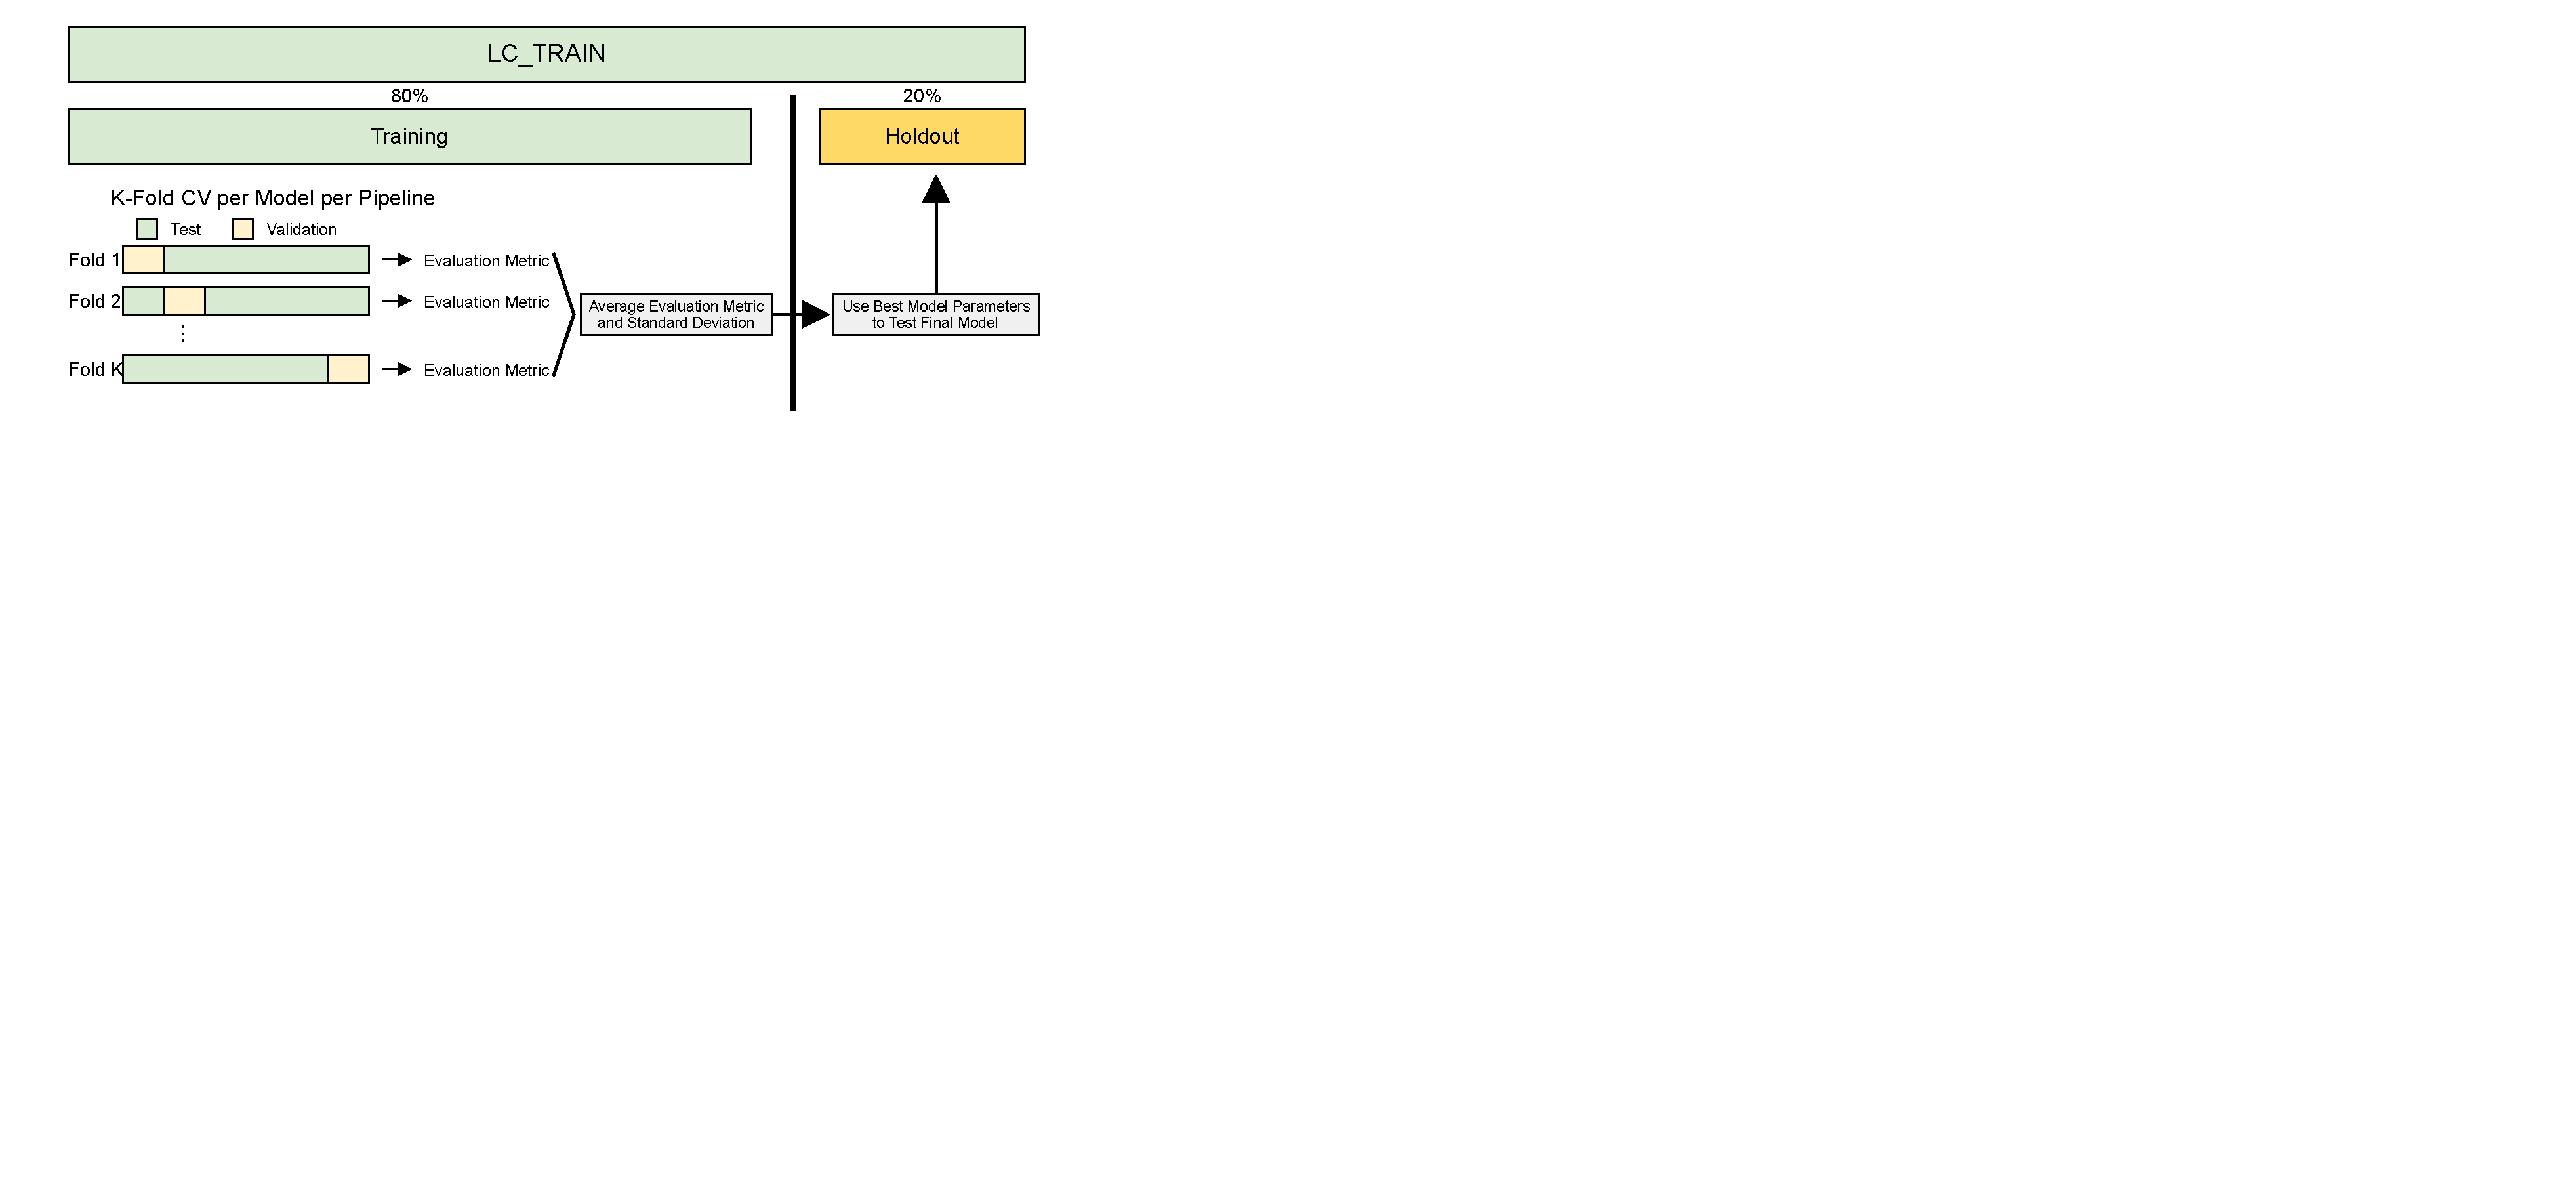
\includegraphics[width=\textwidth]{images/modeling/model_building.pdf}
% \end{frame}

\section{Evaluation}

\begin{frame}
    \frametitle{Best Model Configurations}
        \begin{columns}[T]
            \column{0.48\textwidth}
            \textbf{Duration Prediction}:
            \vspace{-0.5cm}
            \begin{center}
            \small
            \begin{tabular}{>{\columncolor{bgsubrown!20}}l l}
            \toprule
            \textbf{Component} & \textbf{Value} \\
            \midrule
            Model & PenalizedSplines \\
            Pipeline & vanilla \\
            CV Method & kfold \\
            RMSE & 59.47 \\
            R² & 0.059 \\
            \midrule
            Ridge $\alpha$ & 14.38 \\
            Spline degree & 3 \\
            Spline knots & 15 \\
            Scaler & RobustScaler \\
            \bottomrule
            \end{tabular}
            \end{center}
                
            \column{0.48\textwidth}
            \textbf{Occupancy Prediction}:
            \vspace{-0.5cm}
            \begin{center}
            \small
            \begin{tabular}{>{\columncolor{bgsubrown!20}}l l}
            \toprule
            \textbf{Component} & \textbf{Value} \\
            \midrule
            Model & PenalizedSplines \\
            Pipeline & vanilla \\
            CV Method & rolling \\
            RMSE & 3.64 \\
            R² & 0.303 \\
            \midrule
            Ridge $\alpha$ & 29.76 \\
            Spline degree & 3 \\
            Spline knots & 15 \\
            Scaler & RobustScaler \\
            \bottomrule
            \end{tabular}
            \end{center}
        \end{columns}
    
        \begin{alertblock}{Key Insight}
            Both tasks achieved best results with PenalizedSplines and vanilla features, though with different CV methods \& regularization.
        \end{alertblock}
    \end{frame}
    
% \begin{frame}
% \frametitle{Duration: Performance on Holdout Set (9 per aggregates)}
%     \begin{columns}
%         \column{0.5\textwidth}
%         \begin{center}
%         \small
%         \begin{tabular}{>{\columncolor{bgsubrown!20}}l r r}
%         \toprule
%         \textbf{CV Method} & \textbf{RMSE} & \textbf{R²} \\
%         \midrule
%         expanding & 60.41 & 0.029 \\
%         rolling & 60.45 & 0.028 \\
%         kfold & 60.51 & 0.026 \\
%         \bottomrule
%         \end{tabular}
%         \end{center}
            
%         \column{0.5\textwidth}
%         \begin{center}
%         \small
%         \begin{tabular}{>{\columncolor{bgsubrown!20}}l r r}
%         \toprule
%         \textbf{Pipeline} & \textbf{RMSE} & \textbf{R²} \\
%         \midrule
%         vanilla & 60.20 & 0.035 \\
%         interact\_select & 60.55 & 0.024 \\
%         pca\_lda & 60.61 & 0.022 \\
%         \bottomrule
%         \end{tabular}
%         \end{center}
%     \end{columns}

%     \vspace{0.2cm}
%     \begin{center}
%     \small
%     \begin{tabular}{>{\columncolor{bgsubrown!20}}l r r r r}
%     \toprule
%     \textbf{Model} & \textbf{RMSE} & \textbf{(std)} & \textbf{R²} & \textbf{(std)} \\
%     \midrule
%     PenalizedSplines & 60.03 & $\pm$ 0.63 & 0.041 & $\pm$ 0.020 \\
%     Ridge & 60.39 & $\pm$ 0.17 & 0.030 & $\pm$ 0.005 \\
%     PenalizedLogNormal & 60.49 & $\pm$ 0.15 & 0.026 & $\pm$ 0.005 \\
%     Lasso & 60.50 & $\pm$ 0.28 & 0.026 & $\pm$ 0.009 \\
%     KNN & 60.85 & $\pm$ 0.54 & 0.014 & $\pm$ 0.018 \\
%     \bottomrule
%     \end{tabular}
%     \end{center}
    
%     \vspace{-0.2cm}
%     \begin{alertblock}{Key Insight}
%         Above tables are aggregates. PenalizedSplines with vanilla features and KFold CV achieved best performance on holdout set.
%     \end{alertblock}
% \end{frame}

\begin{frame}
\frametitle{Duration: Best Model Diagnostics}
    \begin{center}
        \noindent\centering
        \vspace{-0.7cm}
        % 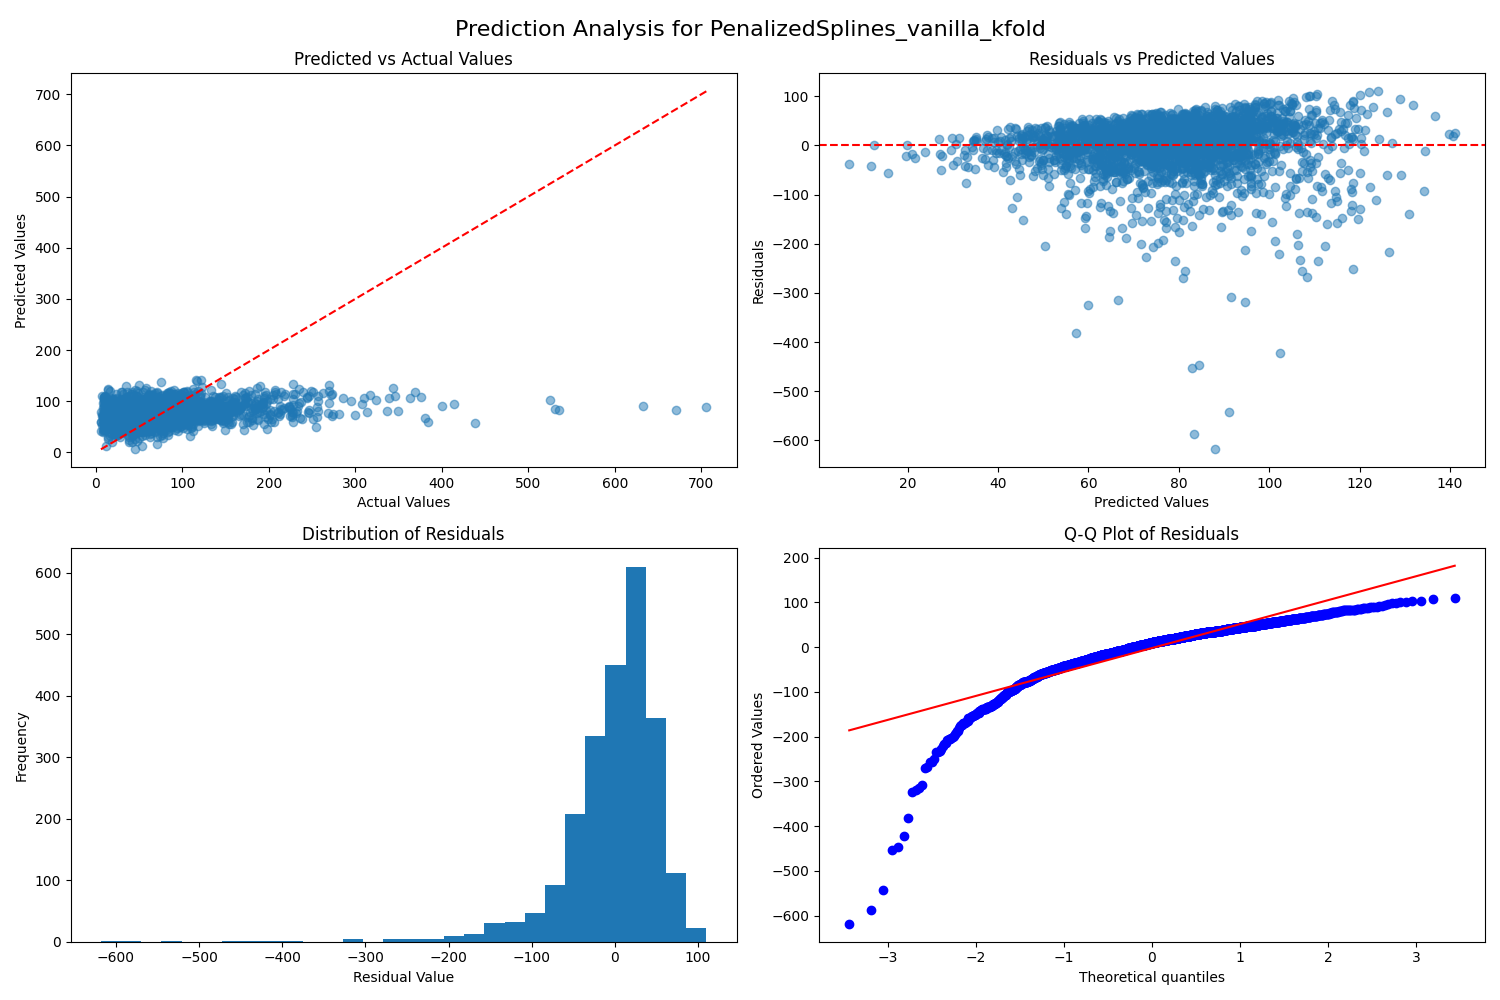
\includegraphics[width=1.0\textwidth, height=0.95\textheight,
        %     % keepaspectratio,    % Maintains aspect ratio
        %     interpolate=false,  % Prevents blurry interpolation
        %     draft=false]{images/evaluation/Duration_PenalizedSplines_vanilla_kfold.jpg}
    \end{center}
\end{frame}

% \begin{frame}
% \frametitle{Occupancy: Performance on Holdout Set}
%     \begin{columns}
%         \column{0.5\textwidth}
%         \begin{center}
%         \small
%         \begin{tabular}{>{\columncolor{bgsubrown!20}}l r r}
%         \toprule
%         \textbf{CV Method} & \textbf{RMSE} & \textbf{R²} \\
%         \midrule
%         expanding & 4.32 & 0.000 \\
%         rolling & 4.34 & -0.021 \\
%         kfold & 4.59 & -0.156 \\
%         \bottomrule
%         \end{tabular}
%         \end{center}
            
%         \column{0.5\textwidth}
%         \begin{center}
%         \small
%         \begin{tabular}{>{\columncolor{bgsubrown!20}}l r r}
%         \toprule
%         \textbf{Pipeline} & \textbf{RMSE} & \textbf{R²} \\
%         \midrule
%         vanilla & 4.04 & 0.138 \\
%         interact\_select & 4.45 & -0.052 \\
%         pca\_lda & 4.76 & -0.263 \\
%         \bottomrule
%         \end{tabular}
%         \end{center}
%     \end{columns}

%     \vspace{0.2cm}
%     \begin{center}
%     \small
%     \begin{tabular}{>{\columncolor{bgsubrown!20}}l r r r r}
%     \toprule
%     \textbf{Model} & \textbf{RMSE} & \textbf{(std)} & \textbf{R²} & \textbf{(std)} \\
%     \midrule
%     PenalizedSplines & 4.00 & $\pm$ 0.50 & 0.150 & $\pm$ 0.231 \\
%     PenalizedWeibull & 4.04 & $\pm$ 0.14 & 0.141 & $\pm$ 0.059 \\
%     Lasso & 4.17 & $\pm$ 0.24 & 0.084 & $\pm$ 0.103 \\
%     PenalizedPoisson & 4.17 & $\pm$ 0.24 & 0.082 & $\pm$ 0.110 \\
%     Ridge & 4.61 & $\pm$ 0.62 & -0.136 & $\pm$ 0.311 \\
%     KNN & 5.51 & $\pm$ 1.29 & -0.675 & $\pm$ 0.829 \\
%     \bottomrule
%     \end{tabular}
%     \end{center}
    
%     \vspace{-0.2cm}
%     \begin{alertblock}{Key Insight}
%         Also aggregates. Vanilla \textit{rolling} PenalizedSplines proved best.
%     \end{alertblock}
% \end{frame}

\begin{frame}
\frametitle{Occupancy: Best Model Diagnostics}
    \begin{center}
        \noindent\centering
        \vspace{-0.7cm}
        % 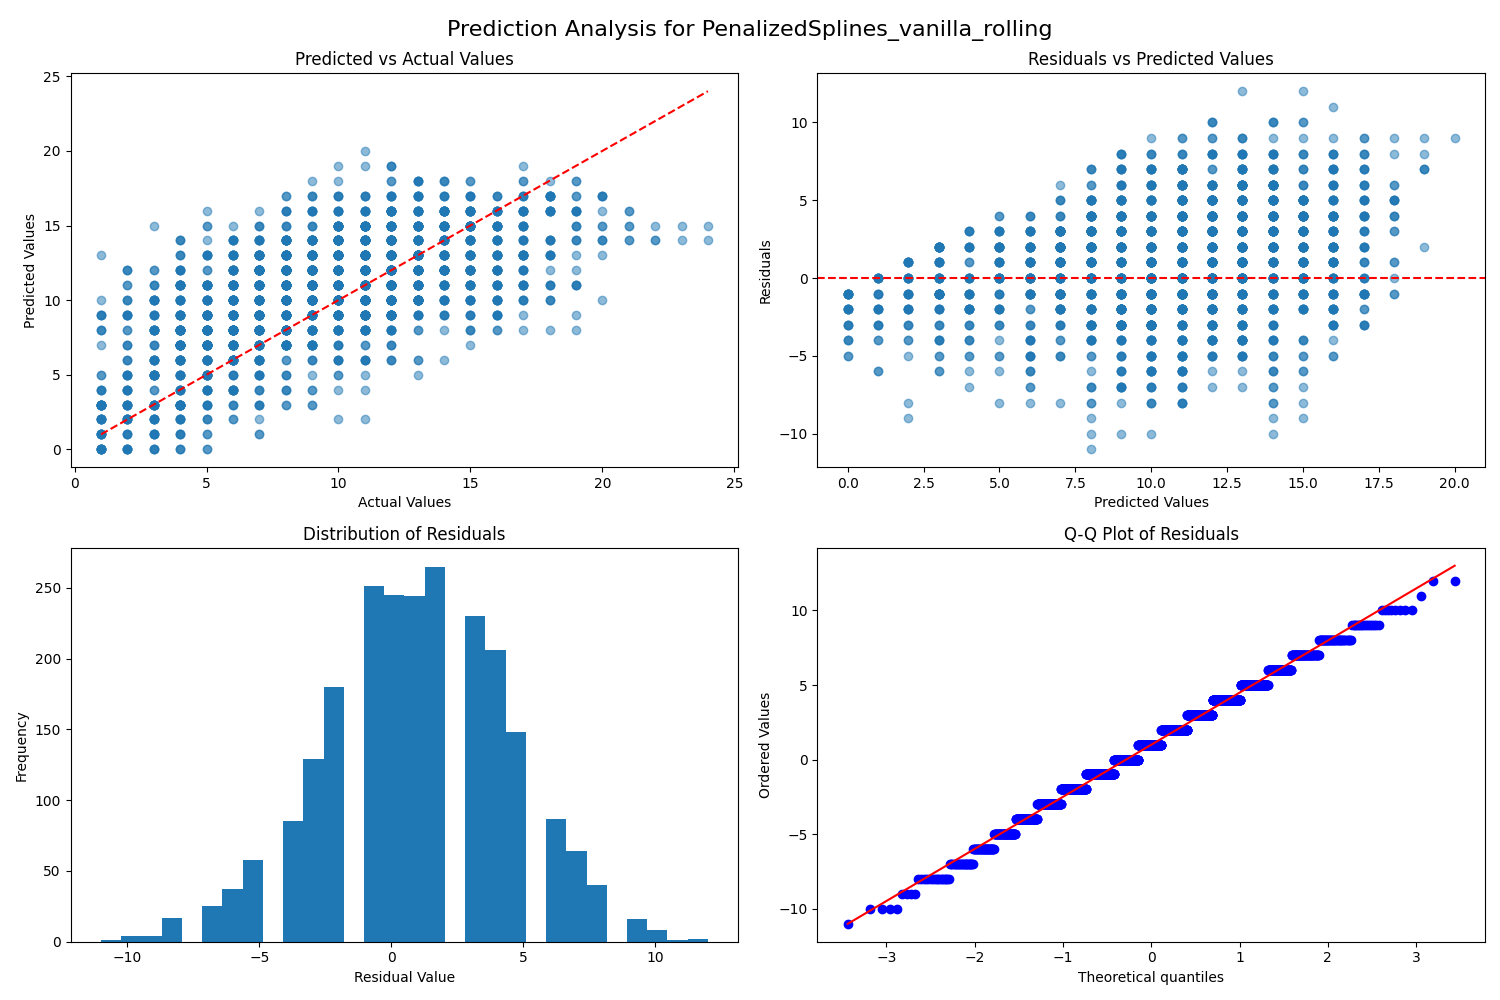
\includegraphics[width=1.0\textwidth, height=0.95\textheight,
        %     % keepaspectratio,    % Maintains aspect ratio
        %     interpolate=false,  % Prevents blurry interpolation
        %     draft=false]{images/evaluation/Occupancy_PenalizedSplines_vanilla_rolling.jpg}
    \end{center}
\end{frame}

\begin{frame}
\frametitle{Sanity Check}
    \vspace{-0.35cm}
    \begin{center}
        % Top image
        % 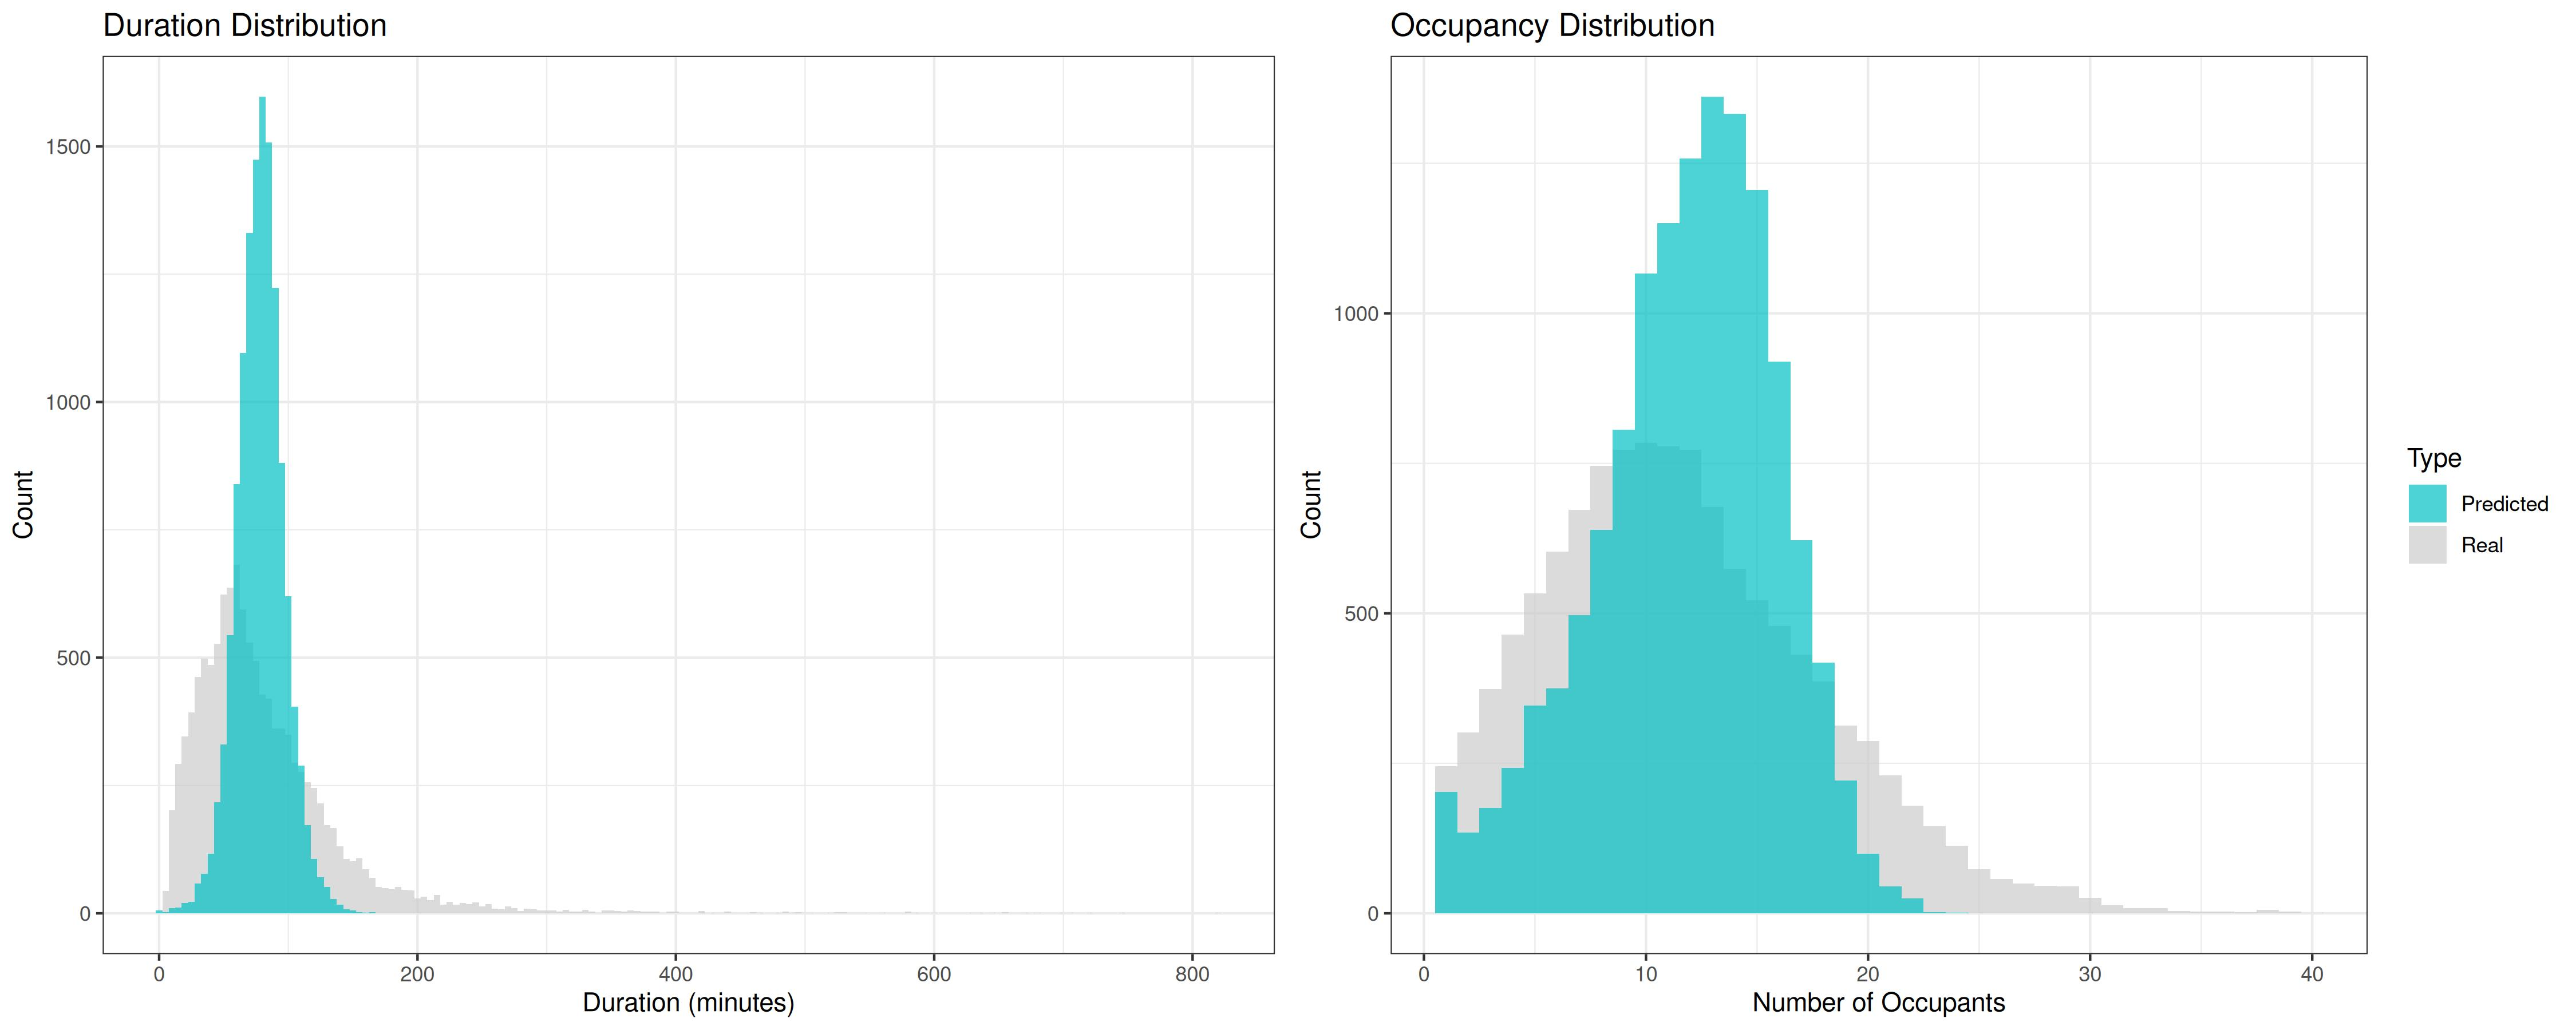
\includegraphics[width=1.0\textwidth, height=0.49\textheight]{images/evaluation/distribution_comparisons.jpg}
        
        \vspace{0.1cm} % Add some vertical spacing between images
        
        % Bottom image
        % 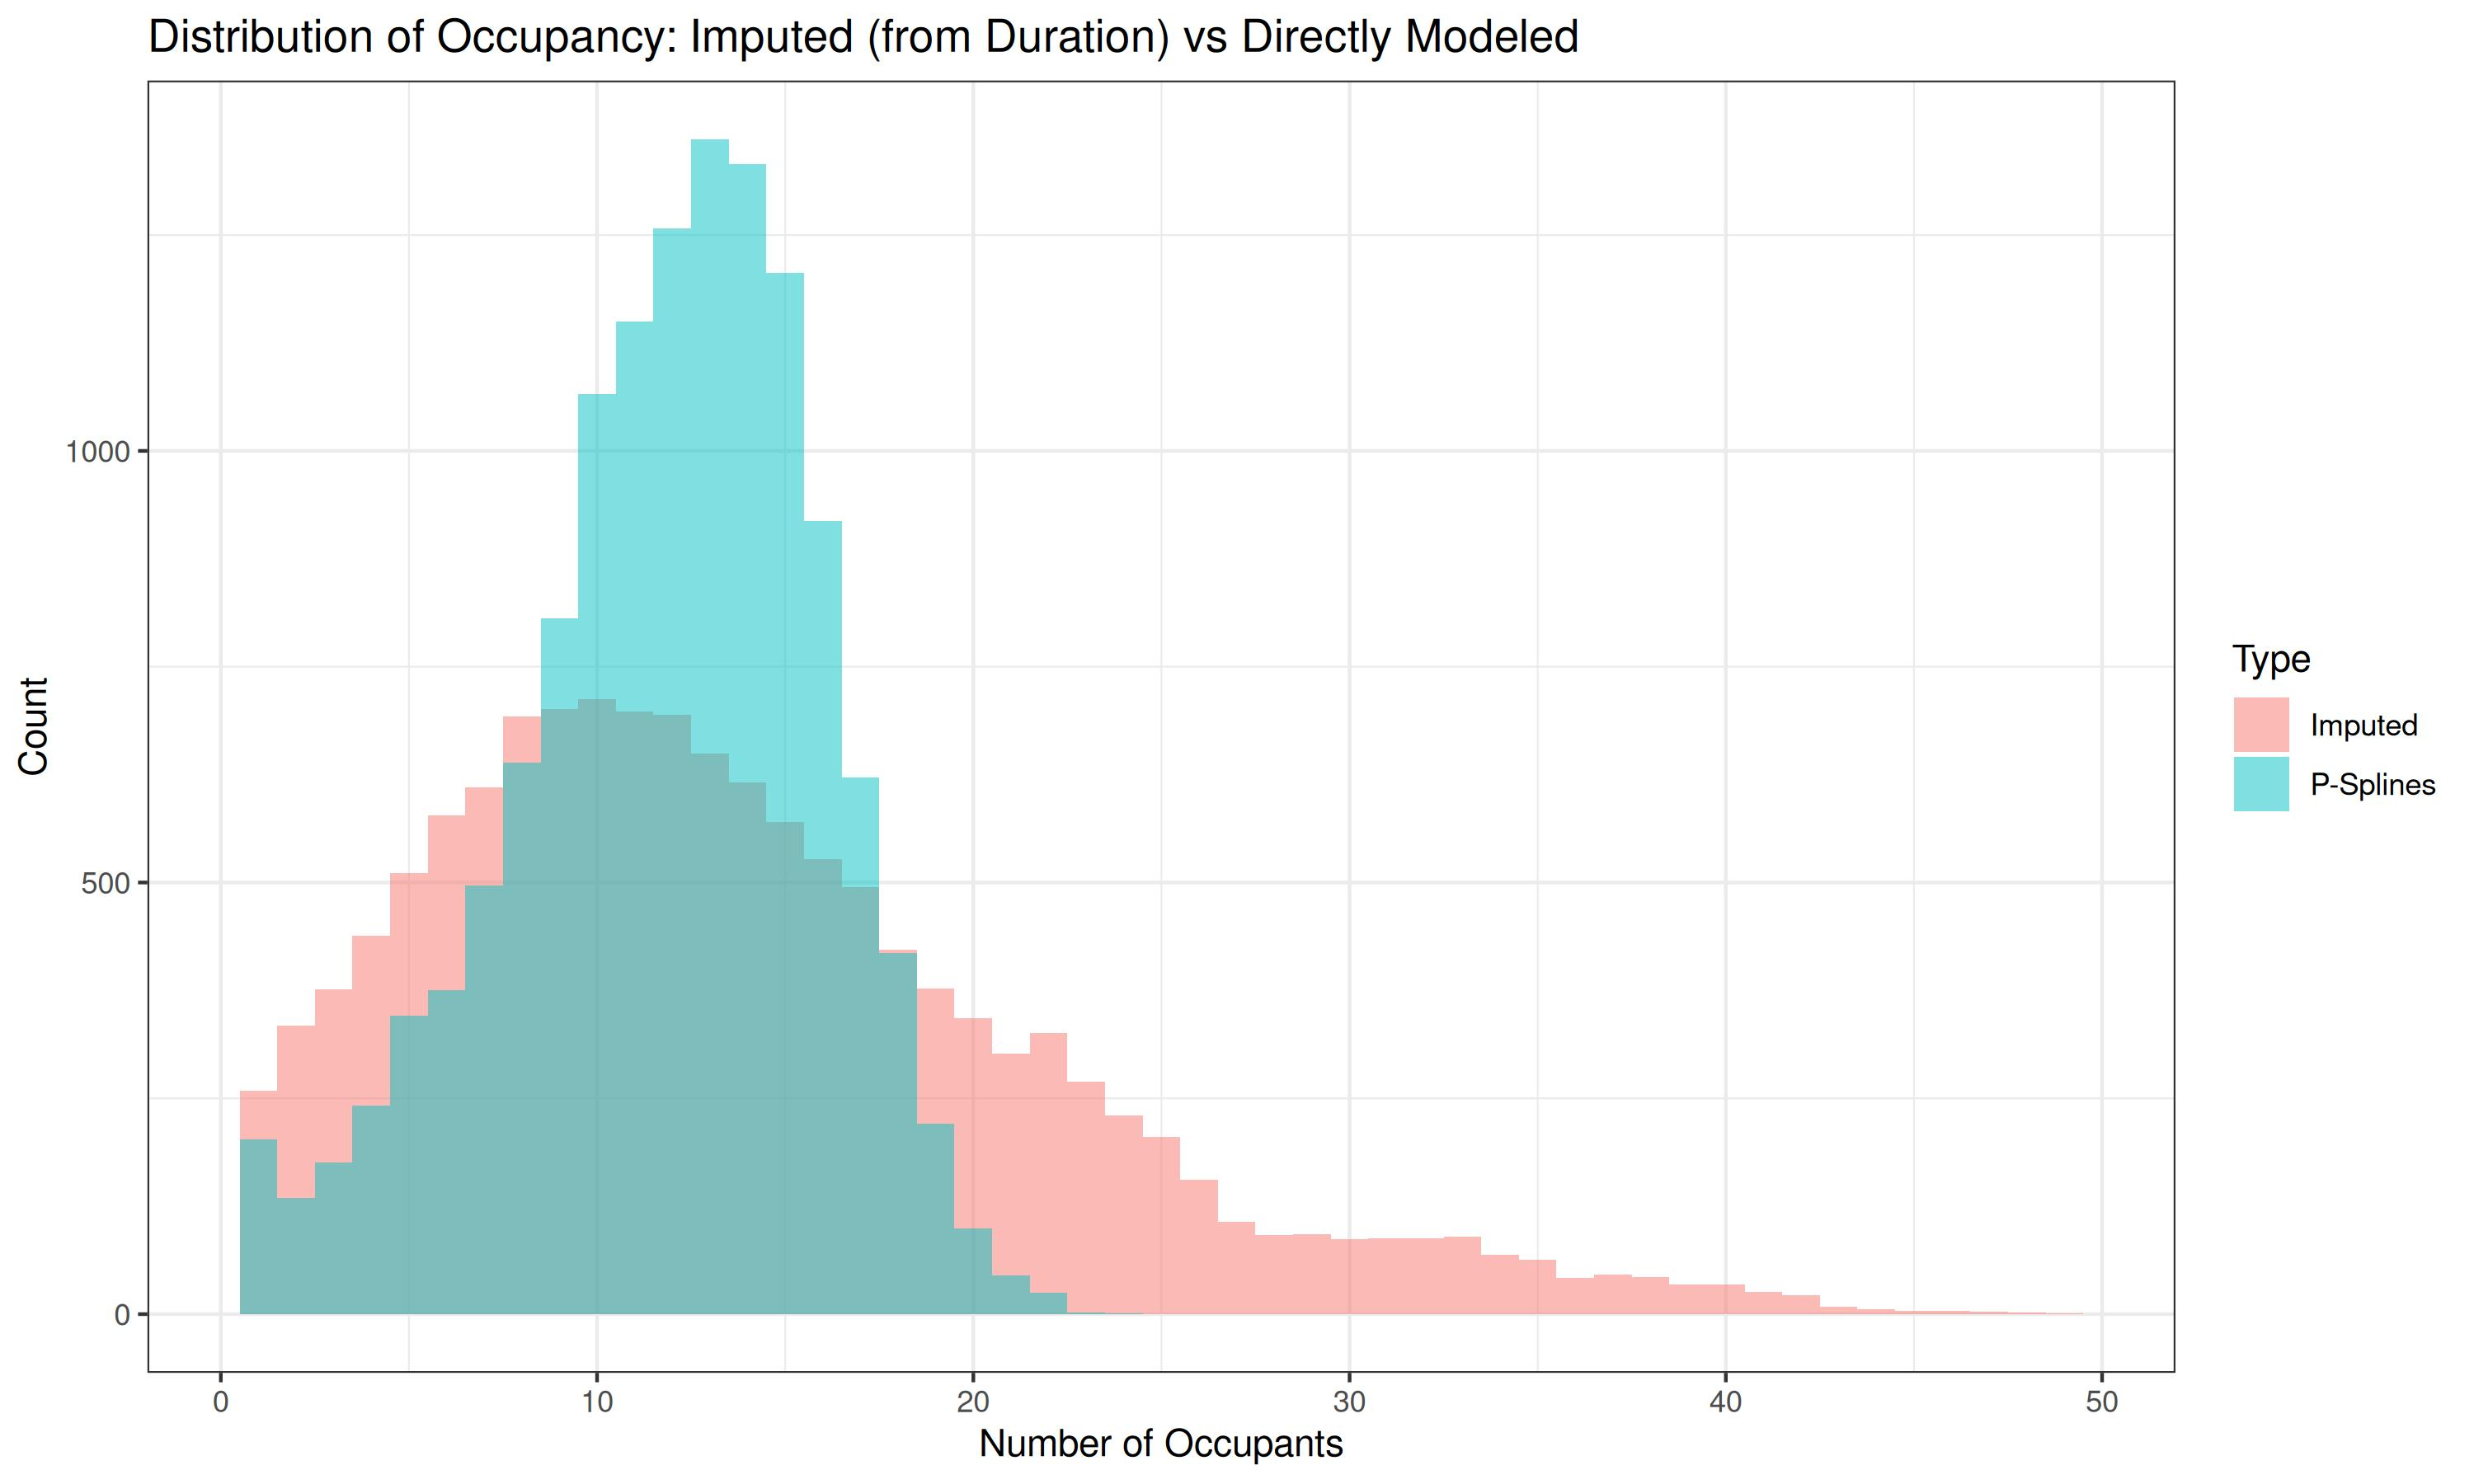
\includegraphics[width=1.0\textwidth, height=0.45\textheight]{images/evaluation/occupancy_comparison_histogram.jpg}

    \end{center}
\end{frame}

\section{Conclusion}

\begin{frame}
\frametitle{Key Findings}
    \begin{columns}
        \column{0.55\textwidth}
        \textbf{Main Results}:
            \begin{itemize}
                \item \textbf{PenalizedSplines} with \textit{vanilla} features performed best
                \item \textbf{Occupancy} prediction shows promise (R² = 0.303)
                \item \textbf{Duration} prediction remains challenging (R² = 0.059)
            \end{itemize}
                            
        \column{0.5\textwidth}
        \textbf{Future Directions}:
            \begin{itemize}
            \item Incorporate \textit{weather} data
            \item Explore \textit{non-linear} relationships further
            \item Investigate \textit{time series} approaches
            \end{itemize}
    \end{columns}

    \vspace{0.5cm}
    \begin{alertblock}{Impact}
        While duration prediction remains difficult, our occupancy model shows strong potential for a victory \textbf{\#CautiousOptimism}
    \end{alertblock}
\end{frame}

\appendix
\begin{frame}[plain]
\begin{center}
    \vspace{-0.5cm}
    \begin{tikzpicture}[remember picture,overlay]
        % Decorative border
        \draw[line width=2pt, bgsubrown] 
            ([shift={(0.5cm,0.5cm)}]current page.south west) 
            rectangle 
            ([shift={(-0.5cm,-0.5cm)}]current page.north east);
        
        \draw[line width=1pt, bgsuorange] 
            ([shift={(0.7cm,0.7cm)}]current page.south west) 
            rectangle 
            ([shift={(-0.7cm,-0.7cm)}]current page.north east);
        
        % Ornamental corners
        \foreach \corner in {north east, north west, south east, south west} {
            \draw[bgsubrown, line width=1.5pt] 
                ([shift={(0.5cm,0.5cm)}]current page.\corner) 
                -- ++(45:0.3cm) -- ++(135:0.3cm);
        }
    \end{tikzpicture}

    \vspace{1cm}
    {\Huge\calligra Thank You}
    \vspace{0.8cm}
    
    \begin{center}
        \begin{tabular}{c}
            {\large\calligra For Your Attention} \\[0.5cm]
            \hline \\[0.1cm]
            {\small Questions \& Discussion Welcome}
        \end{tabular}
    \end{center}
\end{center}
\end{frame}

\end{document} 